%%%%%%%%%%%%%%%%%%%%%%%%%%%%%%%%%%%%%%%%%%%%%%%%%%%%%%%%%%%%%%%%%%%%%%%
%
%   Presentation of Beamer UNL Theme
%   Beamer Presentation by Chris Bourke
%
%%%%%%%%%%%%%%%%%%%%%%%%%%%%%%%%%%%%%%%%%%%%%%%%%%%%%%%%%%%%%%%%%%%%%%%

\documentclass{beamer}

\usetheme[hideothersubsections]{UNLTheme}


\title{Performance Modeling and
Design of Computer Systems- Ch 2 \\
Queueing Theory Terminology}
\author{Debobroto Das Robin} %
\institute{Kent State University}
\date{Spring 2020}

\begin{document}

%{% open a Local TeX Group
%\setbeamertemplate{sidebar}{}
\begin{frame}
        \titlepage
        \begin{center}
    \href{mailto:drobin@kent.edu}{\color{blue}{\texttt{drobin@kent.edu}}}
        \end{center}
\end{frame}
%}% end Local TeX Group

\begin{frame}
\frametitle{Overview} % Table of contents slide, comment this block out to remove it
\tableofcontents % Throughout your presentation, if you choose to use \section{} and \subsection{} commands, these will automatically be printed on this slide as an overview of your presentation
\end{frame}
\section{Classification of Queueing Networks}

\begin{frame}
    \frametitle{Classification of Queueing Networks}
    \framesubtitle{\textbf{\textit{Open Networks}}}
	\begin{itemize}
		\item open queueing network has external arrivals and departures
		\item Example
			\begin{itemize}
			\item CPU uses a time-sharing scheduler to serve a queue of jobs waiting for CPU time
			\item Router in a network serves a queue of packets waiting to be routed.
			\end{itemize}
		\item Queueing theory is built on  \textbf{\textit{stochastic modeling and analysis}} 						\begin{itemize}
					\item Model and analyze  service demands of jobs and the interarrival times of 							jobs as random 	variables. 
				\end{itemize}		  
	\end{itemize}	    
    
\end{frame}

\begin{frame}
    \frametitle{Open Networks: Example}
    \framesubtitle{\textbf{\textit{Network of Queues with Probabilistic Routing}}}
	\begin{itemize}
		\item Server $i$ receives external arrivals (“outside arrivals”) with rate $r_i$ .
		\item Server i also receives internal arrivals from some of the other servers. 
		\item A packet that finishes service at server $i$ is next routed to server $j$ with 							probability $p_{ij}$ . 
		\item Multiple \textbf{“class”} of the packet, may have different probability according to 			routing scheme
		 \begin{figure}
        		\begin{center}
		            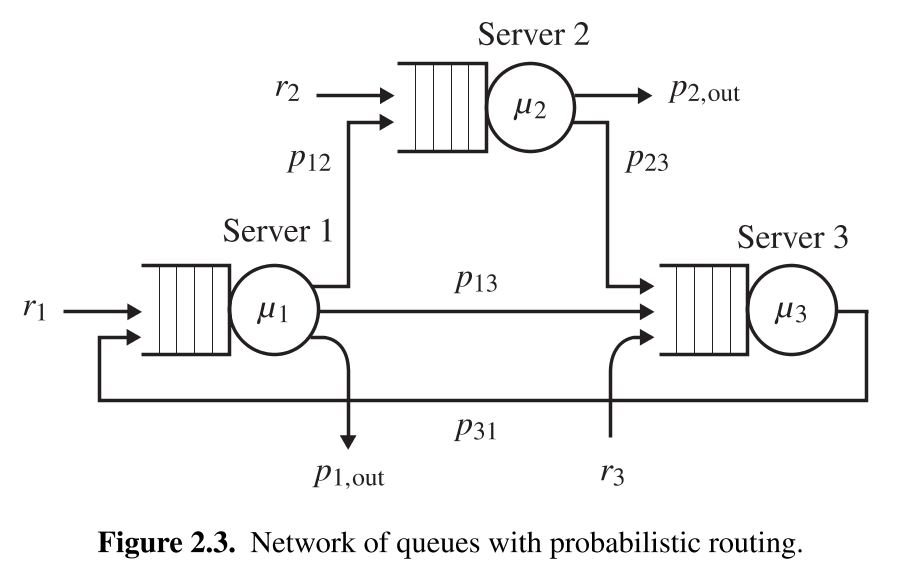
\includegraphics[scale=0.2]{images/Networkqueueswithprobabilisticrouting.jpg}
					%\caption{Sample caption.}
        		\end{center}
		    \end{figure}
		  
	\end{itemize}	    
    
\end{frame}

\begin{frame}
    \frametitle{Open Networks: Example}
    \framesubtitle{\textbf{\textit{Network of Queues with Probabilistic Routing}}}
	\begin{itemize}
			
		\item Real application in internet
			\begin{itemize}
			\item Wire delay can be  replaced by a server with some rate matching with dire delay
			\item \textbf{Goal}: is to predict RTT
			\item \textbf{Deterministic Varation}: instead of $P_{ij}$, specific path to next 						server
			\end{itemize}
			\begin{figure}
        		\begin{center}
		            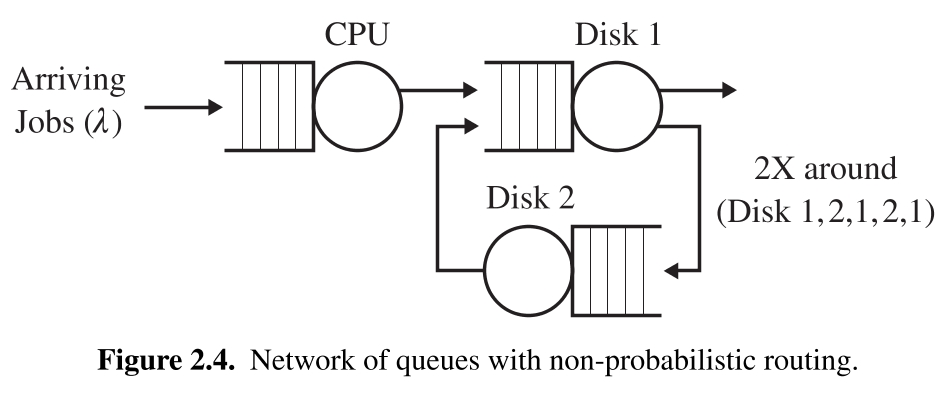
\includegraphics[scale=0.3]{images/deterministicopenqueue.jpg}
					%\caption{Sample caption.}
        		\end{center}
		    \end{figure}
		  
	\end{itemize}	    
    
\end{frame}




\begin{frame}
    \frametitle{Goal of Queueing Theory}
    \framesubtitle{\textbf{\textit{2 Goals}}}
	\begin{itemize}
		\item Predicting the system perfor- mance. Ex. 
		\begin{itemize}
			\item predicting mean delay or delay variability in service   
			\item number of jobs that will be in queue 
			\item mean number of servers being utilized
			\end{itemize}
		\item Developing design of improved system
		\item Example
			\begin{itemize}
			\item Can we build a better system from 1 slow discs or one faster disc
			\item 
			\end{itemize}
	\end{itemize}	    
    
\end{frame}



    
\end{document}